
\mode<presentation>
{
  \usetheme{CambridgeUS}
  \usecolortheme{whale}
  \usecolortheme{lily}

  \setbeamercovered{transparent}
  \usefonttheme[onlymath]{serif}
}

\title[\ReferenceSteadyStateErrorShortName] % (optional, use only with long paper titles)
{\course: \ReferenceSteadyStateErrorName\license}

\subtitle
{Lecture \ReferenceSteadyStateErrorNumber} % (optional)


\begin{document}

\begin{frame}
  \titlepage
\end{frame}

\mode<article>{
\maketitle
\tableofcontents
}


\section{Pre-requisite Material}
This lecture assumes that the reader is familiar with the following material:
\begin{itemize}
\item Lecture \SolvingDifferentialEquationsIINumber:~\SolvingDifferentialEquationsIIName
\item Lecture \BlockDiagramsNumber:~\BlockDiagramsName
\end{itemize}

\section{Reference Input Tracking}

One major reason to implement a control system is to get the system output to follow a prescribed {\em reference trajectory}. A typical control configuration would be the following

\begin{frame}{Feedback Control Configuration}
\begin{center}
\input{figures/controlblockdiagram.tex}
\end{center}
\end{frame}

Here $R(s)$ is the reference trajectory or command trajectory, $Y(s)$ is the system output, and $E(s)$ is the error between the reference and the output. This is fed into the controller $C(s)$, which decides on the actuator commands to the plant under control, $G(s)$.

The controller will be designed to meet many specifications, for example, the closed loop system from $R(s)$ to $Y(s)$ has to be stable, and there may be specific specifications in terms of rise time, settling time, or overshoot for a step command. But we also have a basic question: if we change the set-point command to 72$^{\circ}$, does the output settle out to 72$^{\circ}$ or something else? Thus, we are also interested in the steady state response to a command signal. This question can be answered using the same tool we used in the last lecture: the final value theorem.

\section{Reference Tracking Analysis}

In this case our question is the following. If the reference signal $r(t)$ is a step input, what is the steady state error $e(t)=r(t)-y(t)$? Fortunately, for unity gain feedback, $E(s)$ appears as the output of the summer. For generic analysis, we can combine the controller with the plant (i.e., all gains in the forward path are combined and represented as $G_F(s)$) and examine the following system:

\begin{frame}{Reference Error Analysis}
\begin{center}
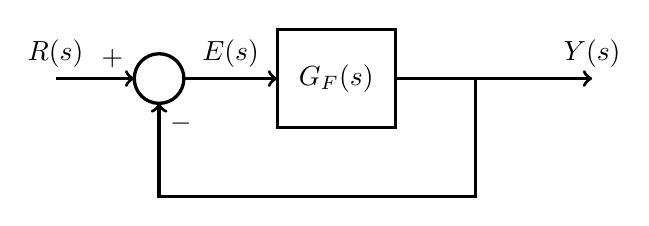
\begin{tikzpicture}[inner sep=0pt,outer sep=0pt,very thick,
sysblock/.style={draw,rectangle,inner sep=2pt,minimum width=1.5cm,minimum height=1.25cm,very thick}]

\draw (0,0) node[draw,circle] (sum) {$\rule{0pt}{18pt}$};
\draw (2.25,0) node[sysblock] (a) {$G_F(s)$};
\draw (4,0) node (c) {};

\draw[<-] (sum.180) node[above left=4pt] {$+$} -- ++(-1,0) node[above=4pt] {$R(s)$};
\draw[->] (sum.0) -- node[pos=.5,above=4pt] {$E(s)$} (a.180);
\draw[->] (a.0) -- ++(2.5,0) node[above=4pt] {$Y(s)$};
\draw[->] (c.0) -- ++(0,-1.5) -| (sum.-90) node[below right=4pt] {$-$};

\end{tikzpicture}
\end{center}
\end{frame}

Since $E(s) = R(s) - Y(s)$, and $Y(s) = \frac{G_F(s)}{1+G_F(s)}R(s)$, 
the transfer function from $R(s)$ to $E(s)$ is
\begin{align*}
E(s) & = R(s) -  \frac{G_F(s)}{1+G_F(s)}R(s)\\
& = \left(1 - \frac{G_F(s)}{1+G_F(s)}\right)R(s)\\
&= \frac{1}{1+G_F(s)}R(s) \\
\end{align*}
In order to apply the final value theorem, a necessary condition is that the Laplace Transform $\frac{s}{1+G_F(s)}R(s)$ has all poles in the left half plane. We will assume this is true. Then the final value theorem tells us that
\[
\boxed{\lim_{t\rightarrow \infty} e(t) = \lim_{s\rightarrow 0} \frac{s}{1+G_F(s)}R(s)}
\]

We will examine the consequences of this for two different inputs

\subsection{Step Input}

If the reference is a step of magnitude $A$, then $R(s)=\frac{A}{s}$. In this case,
\begin{align*}
\lim_{t\rightarrow \infty} e(t) &= \lim_{s\rightarrow 0} \frac{s}{1+G_F(s)}\frac{A}{s} \\
& =  \frac{A}{1+G_F(0)} \\
& = \frac{A}{1+K_{s}}
\end{align*}
Where $K_{s}=G_F(0)$. Conclusion: In order to have a small steady state error, the value $G_F(0)$ should be large. We will see later that this corresponds to the {\em DC gain} of $G_F(s)$, so we can say that a small steady state error requires a large DC gain. If $G_F(s)$ were to have a pole at $s=0$, (which is usually termed as "$G_F(s)$ contains a pure integrator") then the steady state error would be zero.

\subsection{Ramp Input}

If the reference is a ramp of slope $A$, then  $R(s)=\frac{A}{s^2}$. In this case,
\begin{align*}
\lim_{t\rightarrow \infty} e(t) &= \lim_{s\rightarrow 0} \frac{s}{1+G_F(s)}\frac{A}{s^{2}} \\
& =  \lim_{s\rightarrow 0} \frac{A}{s+sG_F(s)}\\
& =   \frac{A}{K_{v}}
\end{align*}
where $K_{v} = \lim_{s\rightarrow 0} sG_F(s)$. For a small steady state error, we need to have $K_{v}$ large. Note that $G_F(s)$ {\em must} contain a pure integrator in order for $K_{v}$ to be nonzero. If we want zero steady state error to a ramp input, then $G_F(s)$ must have two pure integrators (i.e. two roots at $s=0$)

\subsection{System Type}

Since the number of integrators is an important factor in steady state error, this has been given a special name. 

\begin{definition} The number of pure integrators a system contains is the {\em system type}
\end{definition}

For example:
\begin{itemize}
\item $\frac{2}{s^2+1}$ is a type 0 system
\item  $\frac{2}{s(s^2+1)}$ is a type 1 system
\item  $\frac{2}{s^2(s^2+1)}$ is a type 2 system
\end{itemize}

This gives us the following table for steady state error

\begin{center}
\begin{tabular}{c|cc|c}
system type & step input $Au(t)$ & ramp input $A t u(t)$ & Error Constants \\\hline
0 & $\frac{A}{1+K_{s}}$ & $\infty$ & $K_{s} = \lim_{s\rightarrow 0}G_F(s)$ \\
1 & 0 & $\frac{A}{K_{v}}$ & $K_{v} = \lim_{s\rightarrow 0 }sG_F(s)$\\
\end{tabular}
\end{center}

\section{Examples}

\begin{example}Consider the following feedback control system

\begin{frame}{Control System}
\begin{center}
\input{figures/example1.tex}
\end{center}
\end{frame}

If the reference input is $r(t)=2u(t)$ where $u(t)$ is a unit step function, what is the steady state error $\lim_{t\rightarrow \infty}e(t)$?\vspace{.1in}\\
\textbf{Solution:} Step 1 is to find the transfer function from $R(s)$ to $E(s)$. This is
\[
\frac{E(s)}{R(s)} = \frac{1}{1+5\frac{2}{s^{2}+3s+5}} = \frac{s^{2}+3s+5}{s^{2}+3s+15}
\]
Step 2 is to apply the input and use the final value theorem. First, we check that the closed loop system is stable, which we do by verifying that $s^{2}+3s+15$ has two roots with negative real part. Then
\begin{align*}
\lim_{t\rightarrow\infty}e(t) &=  \lim_{s\rightarrow 0} sE(s) \\
&= \lim_{s\rightarrow 0} s\frac{s^{2}+3s+5}{s^{2}+3s+15}\frac{2}{s}\\
&=  \frac{5(2)}{15} = \frac{10}{15}
\end{align*}
\end{example}

If we would like the steady state error to be smaller, we can increase the DC gain, or add an integrator.

\begin{example} Consider the same system as above, but find the steady state error when $r(t)=tu(t)$ (a ramp).\vspace{.1in}\\
\textbf{Solution:} We have already found the transfer function to $E(s)$, so we just need to apply the final value theorem
\begin{align*}
\lim_{t\rightarrow\infty}e(t) &=  \lim_{s\rightarrow 0} sE(s) \\
&= \lim_{s\rightarrow 0} s\frac{s^{2}+3s+5}{s^{2}+3s+15}\frac{1}{s^{2}}\\
&= \lim_{s\rightarrow 0}  \frac{s^{2}+3s+5}{(s^{2}+3s+15)s}\\
& = \infty
\end{align*}
The steady state error is infinite! To check this, let's find the response using \textsc{Matlab}. The closed loop response is 
\[
\frac{Y(s)}{R(s)} = \frac{\frac{10}{s^{2}+3s+5}}{1+\frac{10}{s^{2}+3s+5}} = \frac{10}{s^{2}+3s+15}
\]
The ramp response of $G_F(s)$ is the same as the step response of $G_F(s)/s$, so we can do the following to simulate:\vspace{.1in}\\
\texttt{sys=tf([10],[1 3 15 0])\\
\rule{0pt}{0pt}[y,t]=step(sys,5)\\
plot(t,t,'b-',t,y,'g-','linewidth',2)\\
legend('reference','system output')}\\

The results are shown below.
\begin{frame}{Ramp Response}
\begin{center}
\includegraphics[width=3in]{figures/example2}
\end{center}
\end{frame}
The system output looks like a ramp, but the difference gets bigger with time.
\end{example}

\begin{example} Things will get better if we increase the system type of the controller. Let's repeat the analysis for the following control system
\begin{frame}{Second Control System}
\begin{center}
\input{figures/example2.tex}
\end{center}
\end{frame}
Note that the product of the control and system is now type 1. To find the steady state error, we first find the transfer function from $R(s)$ to $E(s)$
\[
\frac{E(s)}{R(s)} = \frac{1}{1+\frac{5}{s}\frac{2}{s^{2}+3s+5}} = \frac{s^{3}+3s^{2}+5s}{s^{3}+3s^{2}+5s+10}
\]
The closed loop is stable since $s^{3}+3s^{2}+5s+10$ has all roots with negative real part (which can be checked using the Routh-Hurwitz criterion). Then for the step input $r(t)=2u(t)$,
\begin{align*}
\lim_{t\rightarrow\infty} e(t) &=  \lim_{s\rightarrow 0} sE(s) \\
&= \lim_{s\rightarrow 0} s\frac{s^{3}+3s^{2}+5s}{s^{3}+3s^{2}+5s+10}\frac{2}{s}\\
&=  \lim_{s\rightarrow 0} \frac{s^{3}+3s^{2}+5s}{s^{3}+3s^{2}+5s+10}2\\
& = 0
\end{align*}
and for the ramp input $r(t)=tu(t)$,
\begin{align*}
\lim_{t\rightarrow\infty} e(t) &=  \lim_{s\rightarrow 0} sE(s) \\
&= \lim_{s\rightarrow 0} s\frac{s^{3}+3s^{2}+5s}{s^{3}+3s^{2}+5s+10}\frac{1}{s^{2}}\\
&=  \lim_{s\rightarrow 0} \frac{s^{2}+3s+5}{s^{3}+3s^{2}+5s+10}\\
& = \frac{5}{10}
\end{align*}

The steady state error to a ramp input is bounded, which is confirmed via simulation below
\begin{frame}{Ramp Response}
\begin{center}
\includegraphics[width=3in]{figures/example2b}
\end{center}
\end{frame}

\end{example}

\section{Lecture Highlights}
The primary takeaways from this article include
\begin{enumerate}
\setlength{\itemsep}{5pt}
\setlength{\parskip}{0pt}
\setlength{\parsep}{0pt}
\item In control systems, we often want a system's output to track a ``reference'' (desired) input trajectory. For example, we may want an automobile to travel at the speed set by the driver in the cruise control system, in which case the reference would be a step input scaled by the value of the desired speed.
\item System Type theory enables us to determine the order (step, ramp...) of the reference input that a system can track with zero error without having to compute the full time-domain response $y(t)$ or apply the Final Value Theorem to $Y(s)$ for each input type separately.
\item System Type theory also enables us to determine the final value of the error $e(t)$ when the system cannot track the reference with zero error.
\item A system's Type is determined by its number of ``pure integrators''; that is, the number of poles equal to zero. A common mistake is to confuse the number of pure integrators with the order of the system; see Definition 1 for some examples.
\end{enumerate}

\section{Quiz Yourself}

\subsection{Questions}

\begin{enumerate}
\setlength{\itemsep}{5pt}
\setlength{\parskip}{0pt}
\setlength{\parsep}{0pt}
\item Determine the smallest steady state error to a step and ramp input achievable for the following control configuration (hint: don't forget about stability.)
\begin{center}
\input{quizfigures/system1.tex}
\end{center}
\end{enumerate}


\subsection{Solutions}
\begin{enumerate}
\setlength{\itemsep}{5pt}
\setlength{\parskip}{0pt}
\setlength{\parsep}{0pt}
\item \rule{0pt}{12pt}\\
\begin{center}
\includegraphics[width=5in]{quizfigures/1soln}\\
\end{center}
\end{enumerate}


\section{Resources}

\subsection{Books}


\begin{itemize}
\item Norman S. Nise, {\em Control Systems Engineering}, Wiley
\begin{itemize}
\item 7th edition: Sections 7.2-7.3
\end{itemize}
\item Richard C. Dorf and Robert H. Bishop, {\em Modern Control Systems}, Pearson
\begin{itemize}
\item 13th edition: Section 4.6
\end{itemize}
\item Gene F. Franklin, J. David Powell and Abbas Emami-Naeini,  {\em Feedback Control of Dynamic Systems}, Pearson
\begin{itemize}
\item 6th and 7th edition: Section 4.2.1
\end{itemize}
\end{itemize}


\subsection{Web resources}

If you find any useful web resources, please contact your instructor.



\end{document}


